\documentclass[12pt,a4paper,twoside,openany,titlepage,final]{book}

\usepackage[dvips]{geometry}
\geometry{textwidth=15cm,textheight=24cm,top=3.5cm}

\usepackage[small,sf]{caption}

\usepackage{sectsty}
\allsectionsfont{\sffamily\raggedright}

\usepackage{lmodern}
\usepackage[T1]{fontenc}
\usepackage{textcomp}

\usepackage{array}
\extrarowheight4pt

\usepackage{supertabular}

% \usepackage{floatflt}

\usepackage{graphicx}

\usepackage{amsmath}
\usepackage{amssymb}
\usepackage{bm}
\usepackage{framed}

\usepackage{multicol}
\premulticols0.0em

\usepackage{fancyhdr}

\pagestyle{fancy}

\bibliographystyle{plain}

\usepackage{makeidx}

\usepackage{color}

\usepackage{subfigure}
\usepackage{wrapfig}
\DeclareGraphicsExtensions{.png, .jpg, .pdf, .eps} 

\definecolor{link_color}{rgb}{0,0,1}
\definecolor{MARK_color}{rgb}{1,0,0}
\definecolor{filename_color}{rgb}{0.6,0.6,0.6}
% This usepackage command MUST BE LAST !!!
% More details on the hyperref package, including an extensive list of global package options
% can be found at http://www.tug.org/applications/hyperref/manual.html
\usepackage[backref           = page,
            colorlinks        = true,
            linkcolor         = link_color,
            menucolor         = link_color,
            citecolor         = link_color,
            urlcolor          = link_color,
            bookmarksnumbered = true,
            hyperindex        = true]{hyperref}
\hypersetup{pdftitle   = {Fit_esp_charges Manual}}

%\pagestyle{headings}
%\pagenumbering{arabic}

\linespread{1.0}

\newcommand{\la}{$\langle$}
\newcommand{\ra}{$\rangle$}
\newcommand{\boldk}{\mbox{\boldmath$k$}}
\newcommand{\boldr}{\mbox{\boldmath$r$}}
\newcommand{\bolds}{\mbox{\boldmath$\sigma$}}
\newcommand{\boldp}{\mbox{\boldmath$p$}}
\newcommand{\boldR}{\mbox{\boldmath$R$}}
\newcommand{\boldE}{\mbox{\boldmath$E$}}
\newcommand{\boldF}{\mbox{\boldmath$F$}}
\newcommand{\boldG}{\mbox{\boldmath$G$}}
\newcommand{\erf}{\mathop{\mathrm{erf}}}
\newcommand{\erfc}{\mathop{\mathrm{erfc}}}
\newcommand{\bfr}{{\bf r}}
\newcommand{\bfrp}{{\bf r'}}
\newcommand{\bfk}{{\bf k}}
\newcommand{\bfq}{{\bf q}}
\newcommand{\bfR}{{\bf R}}
\newcommand{\bfRp}{{\bf R'}}
\newcommand{\bfRpp}{{\bf R''}}

\renewcommand{\floatpagefraction}{0.75}

% don't like something in the Manual? \MARK{} it and readers will definitely notice!
\newcommand{\MARK}[1]{\textbf{\color{MARK_color} #1}}

\newcommand{\keyword}[1]
{\hyperlink{#1}{\texttt{#1}}}

\newcommand{\subkeyword}[2]{\hyperlink{#1 #2}{\texttt{#2}}}

\newcommand{\option}[1]{\texttt{#1}}


% use this to define a keyword, automatically creates all the links here.
\newcommand{\keydefinition}[3]
{
\centerline{\rule{1.0\textwidth}{1pt}}
\hypertarget{#1}{\textbf{Tag: \texttt{#1}}{ \color{filename_color} (#2)}}
\index{#1@\texttt{#1}}
\\[2ex] \hspace*{0.05\textwidth}
\begin{minipage}{0.92\textwidth}
  #3
\end{minipage} \\
}

\newcommand{\subkeydefinition}[4]
{
\centerline{\rule{1.0\textwidth}{1pt}}
\hypertarget{#1 #2}{\textbf{\keyword{#1} sub-tag: \texttt{#2}} { \color{filename_color} (#3)}}
\index{#1@\texttt{#1}!#2@\texttt{#2}}
\\[2ex] \hspace*{0.05\textwidth}
\begin{minipage}{0.92\textwidth}
  #4
\end{minipage} \\
}

\newcommand{\keydefinitiontwo}[4]
{
\centerline{\rule{1.0\textwidth}{1pt}}
\hypertarget{#1}{\textbf{Tags:\ \texttt{#1}}{ \color{filename_color} (#3)}}
\hypertarget{#2}{\textbf{\newline\phantom{Tags:}\ \texttt{#2}\phantom{a}}{ \color{filename_color} (#3)}}
\index{#1@\texttt{#1}}
\index{#2@\texttt{#2}}
\\[2ex] \hspace*{0.05\textwidth}
\begin{minipage}{0.92\textwidth}
  #4
\end{minipage} \\
}

\newcommand{\keydefinitionthree}[5]
{
\centerline{\rule{1.0\textwidth}{1pt}}
\hypertarget{#1}{\textbf{Tags:\ \texttt{#1}}{ \color{filename_color} (#4)}}
\hypertarget{#2}{\textbf{\newline\phantom{Tags:}\ \texttt{#2}}{ \color{filename_color} (#4)}}
\hypertarget{#3}{\textbf{\newline\phantom{Tags:}\ \texttt{#3}}{ \color{filename_color} (#4)}}
\index{#1@\texttt{#1}}
\index{#2@\texttt{#2}}
\index{#3@\texttt{#3}}
\\[2ex] \hspace*{0.05\textwidth}
\begin{minipage}{0.92\textwidth}
  #5
\end{minipage} \\
}


\makeindex
\begin{document}
\begin{center}
 \begin{Large}
 ESP charges
\end{Large}
\end{center}
This manual describes how to calculate partial charges by fitting to the electro static potential (ESP). These charges are 
widely used in the context of force fields (\cite{Momany1978}, \cite{Cox1981}, \cite{Singh1984}, \cite{Besler1990}, CHELP: 
\cite{Chirlian1987}, CHELPG: \cite{Breneman1990}, RESP-charges: \cite{Bayly1993}, CHELP-BOW/CHELMO: \cite{Sigfridsson1998}, 
ESP-charge from multi-pole-moments: \cite{Hu2007}). This program (Fit\_esp\_charges) implements a simple method for cluster calculation (molecules) as well as 
a method for solids (periodic boundary conditions) \cite{Chen2010}.\\
The starting point for these methods is the calculation of the electro static potential at a sufficiently high number of grid points 
outside the vdw radius of the atoms. To define a space region for the grid two parameters are necessary: a minimal radius and a
maximal radius around the atoms. These radii are defined as multiples of the vdw-radius of the atoms, see figure \ref{esp_radius} 
for details. The values for the vdw radii of most atoms in the periodic table have been taken from 
"http://de.wikipedia.org/wiki/Van-der-Waals-Radius" (\cite{Bondi1964}, \cite{Rowland1996}, \cite{Mantina2009}). For the generation 
of the points cubic grids, provided by a cube-file, are used. For cluster calculations points within the cube encapsulating the spheres with the maximal radius (multiple of the vdw radius) around all atoms are used. For periodic boundary conditions the provided unitcell is used. The points within the superposition of the spheres with the minimal radius (minimal multiple of the vdw radius) are excluded.\\
\begin{figure}[h]
\begin{center}
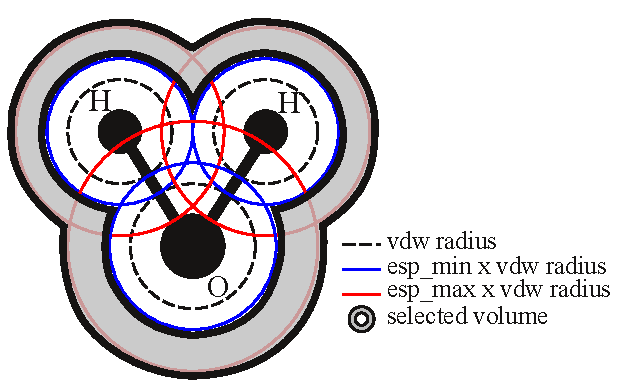
\includegraphics[height=9 cm]{esp_radius}
\end{center}
\caption{Definition of the volume used for the creation of grid points at which the potential is evaluated.} 
\label{esp_radius}
\end{figure}
For the cluster case the function to fit to is a sum of Coulomb potentials with charges $q_i$, the ESP-charges, 
at the atomic position $\mathbf{R}_i$:
\begin{equation}
 V_{ESP}(\mathbf{r})=\sum_{i=1}^{N_{at}}\frac{q_i}{|\mathbf{r}-\mathbf{R}_i|}
\end{equation}
The $q_i$ are calculated by a least squares fit with the additional constraint of constant total charge $q_{tot}=\sum_{i=1}^{N_{at}} q_i$. 
We use the method of Lagrange multipliers to minimize the function:
\begin{equation}
 F=\sum_{k=1}^{N_{grid}}\left(V_{DFT}(\mathbf{r_k})-V_{ESP}(\mathbf{r_k})\right)^2-\lambda\left(q_{tot}-\sum_{i=1}^{N_{at}}q_i\right)^2.\label{F_esp}
\end{equation}
This can be translated into a system of linear equations:
\begin{equation}
 \mathbf{\hat{A}}\mathbf{q}=\mathbf{B}.
\end{equation}
with the $N_{at+1}$ x $N_{at+1}$ matrix $\mathbf{\hat{A}}$:
\begin{align}
A_{ij}=&\sum_{k=1}^{N_{grid}}\frac{1}{|\mathbf{r_k}-\mathbf{R}_i|}\frac{1}{|\mathbf{r_k}-\mathbf{R}_j|}\quad \mathrm{with}\quad i,j\leq N_{at}\\
A_{i=N_{at}+1,j}=&A_{i,j=N_{at}+1}=1;\qquad A_{i=N_{at}+1,j=N_{at}+1}=0\nonumber
\end{align}
and the $N_{at}+1$ vector $\mathbf{B}$:
\begin{align}
 B_i=&\sum_{k=1}^{N_{grid}}\frac{V_{DFT}(\mathbf{r_k})}{|\mathbf{r_k}-\mathbf{R}_i|}\quad \mathrm{with}\quad i\leq N_{at}\\
 B_{i=N_{at}+1}=q_{tot}
\end{align}
$\mathbf{q}$ are the $N_{at}$ charges.\\
For solids (periodic boundary conditions) the situation is more complicated because all charges are repeated infinitely and the 
potential is only defined up-to an arbitrary offset. The methods to solve this problem are based on Ewald summation. 
Details on can be found here \cite{Chen2010}. The function for the potential 
generated by the ESP charges centered at the atoms of the unit-cell now reads:
\begin{equation}
 V_{ESP}(\mathbf{r})=\sum_{i=1,\mathbf{T}}^{N_{at}}q_i\frac{\mathrm{erfc}(\alpha|\mathbf{r}-\mathbf{R_{i,\mathbf{T}}}|)}{|\mathbf{r}-\mathbf{R_{i,\mathbf{T}}}|}+\frac{4\pi}{V_{cell}}\sum_{i=1,\mathbf{k}}^{N_{at}}q_i\mathrm{cos}(\mathbf{k}(\mathbf{r}-\mathbf{R}_{i}))\frac{\mathrm{exp}^{-\frac{k^2}{4\alpha^2}}}{k^2}\label{V_Ewald}
\end{equation}
with $\mathbf{T}=n_1\mathbf{a}_1+n_2\mathbf{a}_2+n_3\mathbf{a}_3$ mapping the lattice positions. $\mathbf{a_i}$ the lattice vectors, 
$n_i \in \mathbb{Z}$. $\mathbf{k}=m_1\mathbf{b}_1+m_2\mathbf{b}_2+m_3\mathbf{b}_3$ mapping the reciprocal space. $\mathbf{b_i}$ the 
reciprocal lattice vectors, $m_i \in \mathbb{Z}$. $V_{cell}$ is the volume of the unit-cell. The parameter $\alpha$ is 
defined as $\alpha=\frac{\sqrt{\pi}}{R_c}$ with $R_c$ the cutoff radius of the Ewald summation. The function to minimize is:
\begin{align}
 F_2^{PBC}=&\sum_{k=1}^{N_{grid}}\left(V_{DFT}(\mathbf{r_k})-\left(V_{ESP}(\mathbf{r_k})+V_{DFT}^{offset}\right)\right)^2\\\nonumber
           &-\lambda\left(q_{tot}-\sum_{i=1}^{N_{at}}q_i\right)+\beta\sum_{i=1}^{N_{at}}\left(q_i-q_{i0}\right)^2. \label{F_esp_pbc2}
\end{align}
The constraint charges $q_{i0}$ can be determined with other methods (e.g. Mulliken charge analysis \cite{Mulliken55}), $\beta$ is the 
weighing factor. This gives $\hat{A}$ and $\mathbf{B}$:
\begin{align}
 &A_{ij}=\sum_{k=1}^{N_{grid}}\left(\frac{\partial V_{ESP}(\mathbf{r_k})}{\partial q_i}\frac{\partial V_{ESP}(\mathbf{r_k})}{\partial q_j}\right)+\beta\delta_{ij} \quad\mathrm{;}\quad i,j\leq N_{at}\\\nonumber
 &A_{i=N_{at}+1,j}=A_{i,j=N_{at}+1}=\sum_{k=1}^{N_{grid}}\frac{\partial V_{ESP}(\mathbf{r_k})}{\partial q_j}\quad j\leq N_{at}\\\nonumber
 &A_{i=N_{at}+2,j}=A_{i,j=N_{at}+2}=1\\\nonumber
 &A_{i=N_{at}+2,j=N_{at}+2}=A_{i=N_{at}+1,j=N_{at}+2}=A_{i=N_{at}+2,j=N_{at}+1}=0\\\nonumber
 &B_{i}=\sum_{k=1}^{N_{grid}}\left(V_{DFT}(\mathbf{r_k})\frac{\partial V_{ESP}(\mathbf{r_k})}{\partial q_i}\right)-\beta q_{0i} \quad \mathrm{;} \quad i\leq N_{at}\\\nonumber
 &B_{i=N_{at}+1}=\sum_{j=1}^{N_{grid}}V_{DFT}(\mathbf{r_j})\\\nonumber
 &B_{i=N_{at}+2}=q_{tot}\nonumber
\end{align}
Here the arbitrary offset of the potential $V_{offset}$ is an additional fitting parameter, the matrix $\hat{A}$ is of dimension $N_{at+2}$ x $N_{at+2}$ and $\mathbf{B}$  of dimension $N_{at+2}$. 
For method 1 $V_{offset}$ can be calculated as:
\begin{equation}
 V_{offset}=\sum_{k=1}^{N_{grid}}\left( V_{DFT} (\mathbf{r_k})-V_{ESP}(\mathbf{r_k})\right)
\end{equation}
from the fitted charges $q_i$. As a measure for the quality of the fit the root-mean-square ($RRMS$) is defined as:
\begin{equation}
 RRMS=\left\{\frac{\sum_{k=1}^{N_{grid}}\left(\left(V_{ESP}(\mathbf{r_k})+V_{offset}\right)-V_{DFT}(\mathbf{r_k})\right)^2}{\sum_{k=1}^{N_{grid}}\left(V_{DFT}(\mathbf{r_k})\right)^2}\right\}^2
\end{equation}
The current implementation is quite sensitive to the points chosen for the calculation of the electrostatic potential. Thorough studies 
regarding the parameters for the grid are advised! For periodic boundary conditions the ESP-charges calculated for transition densities 
are experimental, caution!! The ESP-charges from transition densities can be benchmarked against the dipole-moments calculated with 
\keyword{compute\_dipolematrix}.\\

Calling syntax: 
\begin{verbatim}
      ./Fit_esp_charges cube_file esp_min esp_max R_c rm km charge 
\end{verbatim}
\textit{cube\_file} is the path to the cube-file containing the potential. The \textit{geometry.in} has to be provided in the calling folder


\begin{itemize}
\item \textit{esp\_min esp\_max} \\
  Select the minimal (esp\_min) and maximal (esp\_max) multiple of the vdw radius to select the volume where the 
  potential is evaluated and the esp charges fitted. Defaults: 3 and 8 for clusters and 1 and 2 for pbc. \textit{esp\_max} should not 
  be larger than smallest lattice vector for pbc and radial gird.
\item \textit{r\_m} \\
  PBC only. Maximum number \textit{r\_m} of multiples of the lattice vectors that are used in the real space sum of the Ewald summation. 
  Default: 7
\item \textit{k\_m} \\
  PBC only. Maximum number \textit{k\_m} of multiples of the reciprocal lattice vectors that are used in the reciprocal space sum of the Ewald summation. 
  Default: 7
\item \textit{R\_c} \\
  PBC only. Real space cutoff radius for the Ewald/Wolf-summation. Default: 20$\mathrm{\AA}$.
\item  \textit{charge} \\
  Total charge of the system.

  \end{itemize}
  
\begin{large}
 Compiling\\
\end{large}

The program requires \textit{openmpi} and \textit{Lapack/Scalapack}. Example makefiles are provided in the program folder. The program paralellizes over the gird points.
\bibliography{esp_charges}
\end{document}